%% cv.tex
%% Copyright 2017 Zeyi Fan
%
% This work may be distributed and/or modified under the
% conditions of the LaTeX Project Public License, either version 1.3
% of this license or (at your option) any later version.
% The latest version of this license is in
%   http://www.latex-project.org/lppl.txt
% and version 1.3 or later is part of all distributions of LaTeX
% version 2005/12/01 or later.
%
% This work has the LPPL maintenance status `maintained'.
%
% The Current Maintainer of this work is Zeyi Fan.
%
% This work consists of only the file cv.tex

\documentclass{article}
\usepackage[top=.4in, bottom=.0in, left=3in, right=0.4in,marginparwidth=2.5in]{geometry}
\usepackage[utf8]{inputenc}
\usepackage{tikz}
\usepackage{xcolor}
\usepackage[absolute,overlay]{textpos}
\usepackage{fontspec}
\usepackage{titlesec}
\usepackage{pstricks}
\usepackage{amssymb}
\usepackage{paralist}

\tolerance=1
\emergencystretch=\maxdimen
\hyphenpenalty=10000
\hbadness=10000

\usepackage[pdfauthor={Cesar Reyes}, pdftitle={Cesar Reyes's Resume}, pdfkeywords={}]{hyperref}
\usepackage{hyperref}

\definecolor{mygray}{gray}{0.95}
\definecolor{lightdark}{gray}{0.55}
\definecolor{dark}{gray}{0.3}
\definecolor{skillbg}{gray}{0.7}

\newcommand{\amount}{5.7in}
\setcounter{section}{-1}

\linespread{1.2}
\pagenumbering{gobble}

\renewcommand{\labelitemi}{$\blacksquare$}
\renewenvironment{itemize}[1]{\begin{compactitem}#1}{\end{compactitem}}

% Helpers
\newcommand\twodigits[1]{%
	\ifnum#1<10 0#1\else #1\fi
}

%\newcommand\hl[1]{{\ralewaysb #1}}
\newcommand\hl[1]{#1}


% Fonts
\newfontfamily\raleway{Raleway}
\newfontfamily\ralewaym{Raleway Medium}
\newfontfamily\ralewaysb{Raleway SemiBold}
\newfontfamily\ralewayb{Raleway Bold}
\newfontfamily\ralewayeb{Raleway ExtraBold}
\newfontfamily\ralewaybb{Raleway Black}

\setmainfont{Raleway}

% Styles
\newcommand{\name}[2]{
	\begin{center}
		\Huge{
			\ralewayeb{#1 #2}
		}
	\end{center}
}

\newcommand{\tagline}[1]{
	\begin{center}
		\large{
			\color{dark}
			\ralewaysb{#1}
		}
		\vspace{.2em}
	\end{center}
}

\renewcommand{\thesection}{\twodigits{\arabic{section}}.}

\titleformat{\section}
[hang]
{\ralewaysb\large\color{dark}}
{}
{.0em}
{}
[{\titlerule[0.8pt]}]

\titlespacing*{\section}{0pt}{4pt}{10pt}

\setlength{\TPHorizModule}{1mm}
\setlength{\TPVertModule}{1mm}
\setlength{\parindent}{0mm}

\newcommand{\contactline}[2]{
	\ralewaysb{#1} & \raleway{#2}
}

\newcommand{\skill}[2]{
	\vspace{.2em}
	\ralewayb{#1}
	
	\psset{xunit=0.197\linewidth, yunit=5pt}
	\begin{pspicture}[showgrid=false](5,1)
	\psline[linecolor=skillbg](0,0.5)(5,0.5)
	\psline[linecolor=skillbg,arrows=|-|](1,0.5)(2,0.5)
	\psline[linecolor=skillbg,arrows=|-|](3,0.5)(4,0.5)
	\psline[linecolor=skillbg,arrows=-|](0,0.5)(5,0.5)
	
	\psline[linecolor=black,arrows=|-|](0,0.5)(#2,0.5)
	\end{pspicture}
}

\newcommand{\block}[3]{
	{\large\ralewayb #1}
	
	\ralewaym{\color{lightdark}#2}
	
	\raleway{#3}
}

\begin{document}
	
	% background
	
	\begin{tikzpicture}[remember picture,overlay]
	\fill[mygray] (current page.south west) rectangle ([xshift=-\amount]current page.north east);
	\end{tikzpicture}
	
	% Side Bar
	
	\begin{textblock}{58.5}(6,7.7)
		\begin{figure}
			\centering
			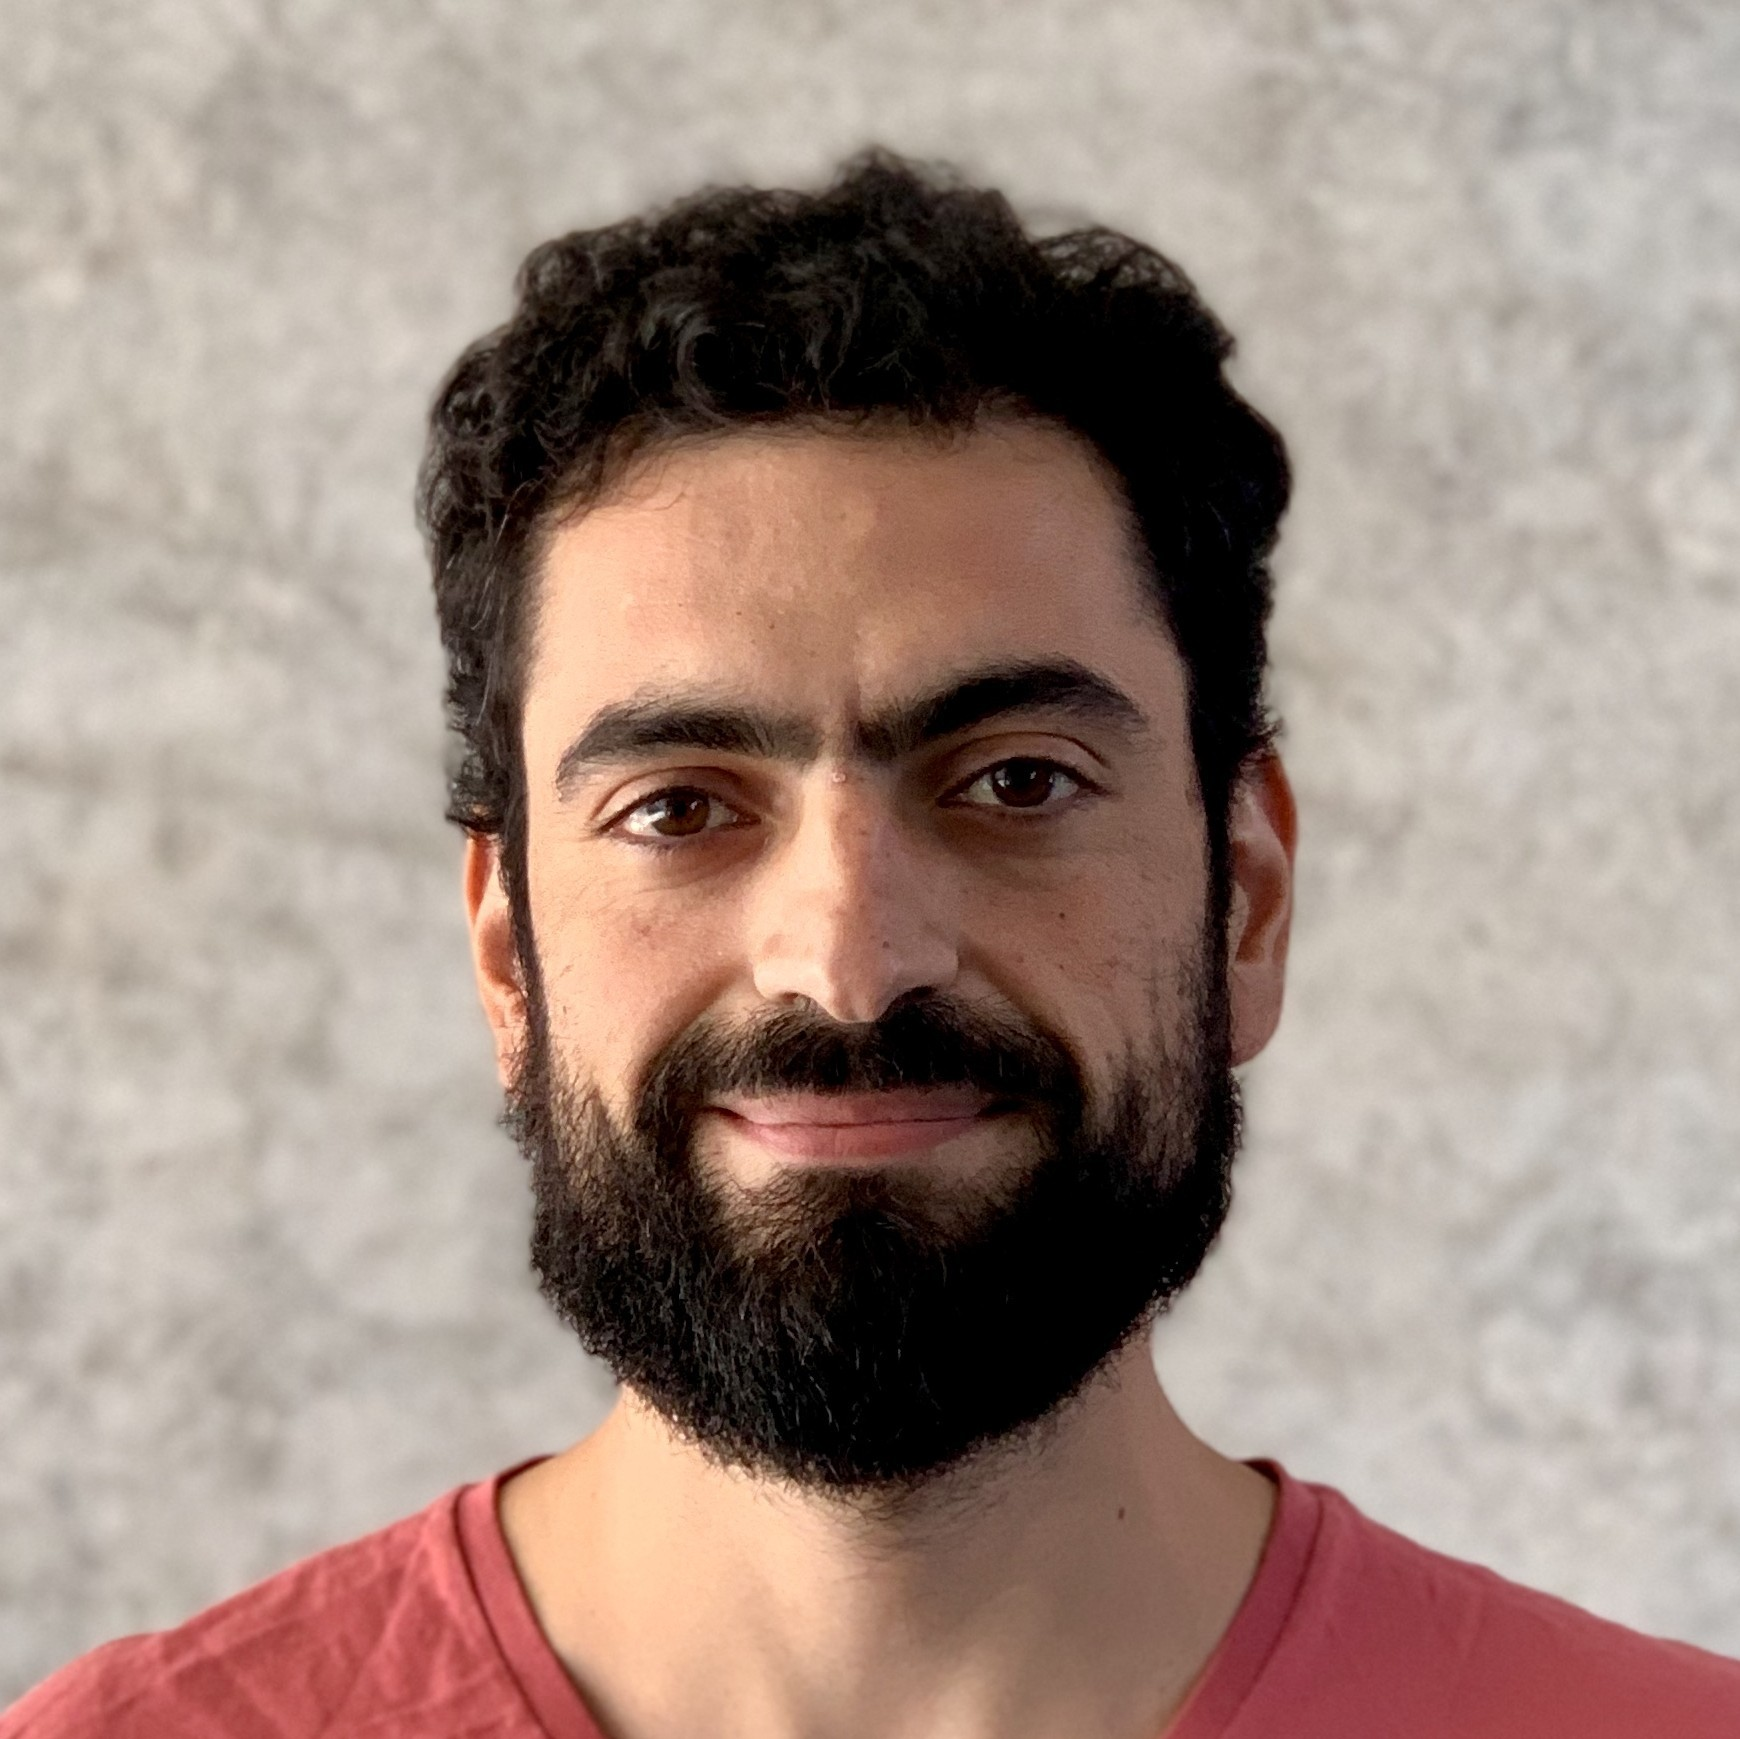
\includegraphics[width=0.8\linewidth]{creyesp.jpg}
		\end{figure}
		
		\name{C\'esar}{Reyes}
		
		\tagline{Data Scientist \& ML engineer}
		
		\section{Resumen}
		
		\color{dark}
		
		Apasionado en ciencia de datos, inteligencia artificial, y el mundo open source. 
		Autodidacta, difusor del conocimiento, docente y Co-organizador de la Meetup de Data Science Montevideo.
		Especial interés en NLP, RecSys y MLOps.
		
		\section{Contacto}
		
		\renewcommand{\arraystretch}{1.1}
		
		\begin{tabular}{rl}
			\contactline{Celular}{(+598) 92716167} \\
			\contactline{Email}{cesar.reyesp@gmail.com} \\
			\contactline{GitHub}{\href{https://github.com/creyesp}{@creyesp}} \\
			\contactline{LinkedIn}{\href{https://linkedin.com/in/creyesp}{/in/creyesp}}
		\end{tabular}
		
		\section{Habilidades}
		
		\textbf{Code}: Python, R, Bash, Git\\
		\textbf{Cloud GCP}:  BigQuery, Storage, PubSub, DataFlow, GCE, Cloud Run, Cloud Build, Vertex AI\\
		\textbf{Frameworks}:  Docker, Airflow, Kubeflow, Apache Beam\\
		\textbf{Data analysis}: Pandas, Numpy, Matplotlib, Seaborn, Bokeh\\
		\textbf{ML}: Scikit-Learn, TensorFlow, Pytorch, Huggingface\\
		\textbf{Serving}: TF Serving, TorchServe, MLServe, FastAPI\\
		\textbf{SO}: GNU/Linux
		
		\section{Idiomas}
		\textbf{Español, Inglés}
		
		
	\end{textblock}
	
	% Main
	
	\vspace{-25pt}  % Change this value to adjust the position of the right
	
	\section{Experiencia Laboral}
	\block{Principal Data Scientist}
	{PedidosYa | Montevideo, Uruguay | Enero 2022 - Actualidad}
	{
		\begin{itemize}
			\item Coordinar y liderar el chapter de Data Scientist en el área de Data
			\item Guiar el desarrollo de nuevos desarrollos de nuevas iniciativas de ML
			\item Líder técnico en el desarrollo de sistemas de recomendación
			\item Colaborar en el desarrollo de la ML Platform interna de la compañía
		\end{itemize}
	}
	
	\vspace{.5em}
	
	\block{Sr Data Scientist}
	{PedidosYa | Montevideo, Uruguay | Enero 2021 - Diciembre 2021}
	{	
		\begin{itemize}
			\item Trabajar con los stakeholders identificando oportunidad y mejoras en los productos usando técnicas de ML.
			\item Desarrollar modelos de ML y llevar estos a producción.
			\item Colaboración con otros DS en puesta en producción de modelos de ML.
		\end{itemize}
	}	
	
	\vspace{.5em}
	
	\block{SSr Data Scientist}
	{PedidosYa | Montevideo, Uruguay | Mayo 2020 - Diciembre 2020}
	{
		
		\begin{itemize}
			\item Desarrollo de modelos de NLP para la detección de la ontología de productos
			\item Desarrollar framework para realizar A/B testing
		\end{itemize}
	}	
	
	\vspace{.5em}
	
	\block{Docente de Machine Learning}
	{Universidad ORT | Montevideo, Uruguay | Octubre 2020 - Actualidad}
	{
		Docente en el Diploma de Especialización en Analítica de Negocios.
		\begin{itemize}
			\item Materia Machine Learning Supervisado en R
		\end{itemize}
		
	}
	
	\vspace{.5em}
	
	
	\block{Co-fundador / Head of Data Science \& Research}
	{Alphalabs | Montevideo, Uruguay | Junio 2020 - Actualidad}
	{
		Co-fundador de AlphaLabs y miembro del área de Data Science
		
		\begin{itemize}
			\item Desarrollo de modelos de ML 
			\item Streaming de datos, Scraping y ETL
			\item Deploy de modelos usando TorchServe y API custom (Fast API)
		\end{itemize}
	}
	
	\vspace{.5em}
	
	\block{Data Scientist}
	{Bluekiri | Montevideo, Uruguay | Enero 2019 - Mayo 2020}
	{
		\begin{itemize}
			\item Análisis descriptivo para la obtención insight para negocio.
			\item Desarrollo de modelos de optimización de precio y predicción de cancelación de reservas
			\item Automatización de procesos con Apache Airflow, Python packages y Azure CI/CD.
		\end{itemize}
	}	
	
	\vspace{.5em}
	
	\block{Research Assistant}
	{Universidad Técnica Federico Santa María | Valparaíso, Chile - Remoto | Abril 2015 – Diciembre 2018}
	{
		Proyecto de Neurociencia Computacional
		\begin{itemize}
			\item Recolección, análisis y procesamiento de señales del sistema visual.
			\item Desarrollo de modelos modelos estadísticos.
			\item Desarrollo del package Spikelib alojado en PyPi.
		\end{itemize}
		
		Publicaciones: \\
		Characterization of Retinal Functionality at different Eccentricities in a Diurnal Rodent \url{https://doi.org/10.1101/277814 }
	}
	\newpage
	\vspace{.5em}
	\section{Educación}
	
	\block{Ingeniero Civil Electrónico con especialidad en Informática}
	{Universidad Técnica Federico Santa María - Titulado 2016}
	{
		Memoria de título profesional: Creación de un módulo en Snort para la detección de intrusos en la red con técnicas estadísticas. Desarrollado en C.
		
	}
	\section{Workshops y talleres}
	\begin{itemize}[-]
		\item Charla: Puesta en producción de modelos de ML - AI Talks - 2021
		\item Workshop: ML usando data de sesiones de apps - Campus Party - 2021
		\item Workshop: Scikit-learn pipelines - Meetup DS/ML Montevideo - 2019
		\item Workshop: ML applicado con Scikit-learn - Quanam - 2019
	\end{itemize}
	
	\section{Actividades de aprendizaje continuo}
	\begin{itemize}[-]
		\item Reinforcement Learning: An Introduction (Book) [On-process] \hfill 2022
		\item Building Machine Learning Pipelines: TFX (book) \hfill 2022
		\item Recommender Systems and Deep Learning in Python (Udemy) \hfill 2021
		\item Building Recommender Systems with Machine Learning and AI (Udemy) \hfill 2021
		\item Machine Learning Design Patterns (Book) \hfill 2021
		\item Deploy Machine learning Model in Production (udemy) \hfill 2020
		\item Full Stack Deep Learning Course \hfill 2020
		\item Hands-On Machine Learning with Scikit-Learn, Keras, and TensorFlow, (book) 2nd Edition \hfill 2020
		\item The Hundred-Page Machine Learning Book (book) by Andriy Burkov \hfill 2019   
		\item Workshop Categorización de Productos con Deep Learning (Mercado Libre) \hfill 2019
		\item PyData Córdoba \hfill 2019
		\item Curso online de data science en python dictado por la Universidad de San Diego, California por el portal EdX (Python for Data Science UCSanDiegoX - DSE200x). \hfill 2018
		\item  Workshop dictado por Tryolabs para la detección de objetos usando TensorFlow.  \hfill Nov 2018
		
	\end{itemize}
	
	\section{Reconocimientos}
	\ralewaysb Primer lugar Dataton. \raleway PedidosYa \hfill 2021
	\ralewaysb Excelencia Académica. \raleway Universidad Técnica Federico Santa María \hfill 2007-2012
	\ralewaysb Mérito Académico. \raleway Departamento de Electrónica - UTFSM\hfill 2007
	
	\section{Otras actividades}
	\ralewaysb 	Co-Organizado de la Meetup Montevideo Applied Data Science and Big Data UY
	
	
\end{document}



